\documentclass{beamer}  
\usetheme{Warsaw}
\usepackage{graphicx}
\title{Introduction to AI and ML}
\subtitle{ Matrix Project}
\author{A.AVINASH, EE17BTECH11005 \and \\K.DEVENDER, EE17BTECH11015}
\begin{document}

\begin{frame}

\titlepage
 
\end{frame}  

\begin{frame}[t]{Q.no.55 in JEE Mains(2005)}
An ellipse has OB as semi minor axis, F and F' its focii and the angle FBF' is a right angle. Then the eccentricity of the ellipse is
\end{frame}
\begin{frame}
Let 'a' be the length of semi major axis.
\newline
Let 'b' be the length of semi minor axis.
\newline
$O(0,0)$ is centre of ellipse
\newline
\Let F and F' are focii
\newline
we know, 
\newline
\[\| OF\| = \sqrt{a^{2}-b^{2}}\]
\newline



\end{frame}
\begin{frame}
Let \textbf{X} be the direction vector of OF 
\newline
\[OF = \sqrt{a^{2}-b^{2}}\textbf{X}\]
 
\ \hspace{30mm}where \|X\| = 1



\[ \hspace{15mm} So,\hspace{5mm} \textbf{X}^{T}\textbf{X} = 1 \hspace{10mm}\textbf{(1)} \]

\newline
Similarly for OF'
\newline
\[OF' = -\sqrt{a^{2}-b^{2}}\textbf{X}\]
As OB is perpendicular to OF and as \|OB\| = b

\end{frame}
\begin{frame}
So,
\newline
\[OB = b\begin{bmatrix}
0 & 1 \\
-1 & 0
\end{bmatrix}\textbf{X}\]
\newline
And also
\newline
\[(OB)^{T}(OF) = 0\] 

\newline
\[\textbf{X}^{T}\begin{bmatrix}
0 & -1 \\
1 & 0
\end{bmatrix}\textbf{X} = 0 \hspace{15mm}\textbf{(2)} \]
\end{frame}
\begin{frame}
We know
\newline
\[BF = OF - OB\]

\implies
 \[BF =  \sqrt{a^{2}-b^{2}} \textbf{X} - b\begin{bmatrix}
0 & 1 \\
-1 & 0
\end{bmatrix}\textbf{X} \]
\newline
\newline
\[BF' = OF' - OB\]

\implies
\[BF' =  -\sqrt{a^{2}-b^{2}} \textbf{X} - b\begin{bmatrix}
0 & 1 \\
-1 & 0
\end{bmatrix}\textbf{X} \] 





\end{frame}
\begin{frame}
As BF is perpendicular to BF', we have
\[(BF)^{T}(BF') = 0\]
\newline
\implies
\[(\sqrt{a^{2}-b^{2}}\textbf{X}^{T} - b\textbf{X}^{T}\begin{bmatrix}
0 & -1 \\
1 & 0
\end{bmatrix})

\hspace{40mm}(-\sqrt{a^{2}-b^{2}}\textbf{X} - b\begin{bmatrix}
0 & 1 \\
-1 & 0
\end{bmatrix}\textbf{X}) = 0\]
\end{frame}



\begin{frame}

\newline
\newline
\newline
\implies
\[-(a^{2}-b^{2})\textbf{X}^{T}\textbf{X} - b\sqrt{a^{2}-b^{2}}\textbf{X}^{T}\begin{bmatrix}
0 & 1 \\
-1 & 0
\end{bmatrix}\textbf{X} + b\sqrt{a^{2}-b^{2}}\textbf{X}^{T}\begin{bmatrix}
0 & -1 \\
1 & 0
\end{bmatrix}\textbf{X} + b^{2}\textbf{X}^{T}\begin{bmatrix}
0 & -1 \\
1 & 0
\end{bmatrix}\begin{bmatrix}
0 & 1 \\
-1 & 0
\end{bmatrix}\textbf{X} = 0\]
\newline
\newline
\newline
\implies
\[-(a^{2}-b^{2}) + b^{2}\textbf{X}^{T}(\textbf{I})\textbf{X}=0\]
\newline



\end{frame}
\begin{frame}


\[2b^{2} = a^{2}\]
\newline


\[\dfrac{b^{2}}{a^{2}} = \frac{1}{2}\]
\newline


\[e=\sqrt{1-\dfrac{b^{2}}{a^{2}}}\]
\newline
\[e=\dfrac{1}{\sqrt{2}}\]
\newline
\ Therefore eccentricity of ellipse =\dfrac{1}{\sqrt{2}}




\end{frame}
\begin{frame}

\begin{figure}
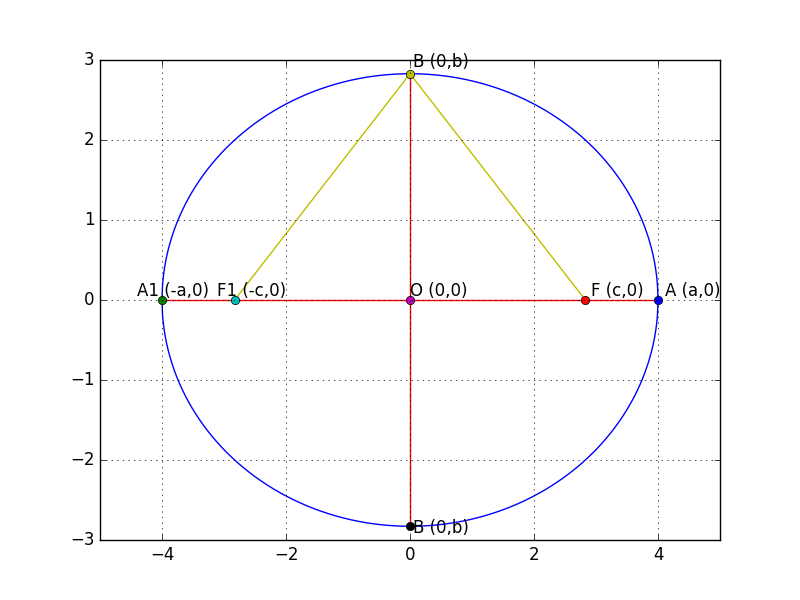
\includegraphics[width=\linewidth]{Avinash.png}
\end{figure}


\end{frame}
\end{document}